\chapter{Advection-Diffusion-Reaction Solver}

%3.4/UserGuide/Tutorial/ADRSolver
%3.4/UserGuide/Examples/ADRSolver/1DAdvection
%3.4/UserGuide/Examples/ADRSolver/3DAdvectionMassTransport
%3.4/UserGuide/Examples/ADRSolver/Helmholtz2D

\section{Synopsis}

The ADRSolver is designed to solve partial differential equations of the form:
\begin{equation}
\alpha \dfrac{\partial u}{\partial t} + \lambda u + \nu \nabla u + \epsilon \nabla \cdot (D \nabla u) = f
\end{equation}
in either discontinuous or continuous projections of the solution field. 
For a full list of the equations which are supported, and the capabilities of each equation, 
see the table below.

\begin{table}[h!]
\begin{center}
\tiny
\renewcommand\arraystretch{2.2} 
\begin{tabular}{llll}
\toprule
\textbf{Equation to solve} & \textbf{EquationType} & \textbf{Dimensions}   &
\textbf{Projections} \\
\midrule
$\nabla^2 u = 0$ & 
    \inltt{Laplace} & All &  Continuous/Discontinuous	\\
$\nabla^2 u  =  f$ & 
    \inltt{Poisson} & All &  Continuous/Discontinuous	\\
$\nabla^2 u  + \lambda u =  f$ & 
    \inltt{Helmholtz} & All & Continuous/Discontinuous \\
$\epsilon \nabla^2 u + \mathbf{V}\nabla u = f$ & 
    \inltt{SteadyAdvectionDiffusion} & 2D only & Continuous/Discontinuous \\
$\epsilon \nabla^2 u +  \lambda u = f$ & 
    \inltt{SteadyDiffusionReaction} & 2D only &  Continuous/Discontinuous \\
$\epsilon \nabla^2 u  \mathbf{V}\nabla u + \lambda u = f$ & 
    \inltt{SteadyAdvectionDiffusionReaction} & 2D only & 
    Continuous/Discontinuous \\
$ \dfrac{\partial u}{\partial t} + \mathbf{V}\nabla u = f$ &
    \inltt{UnsteadyAdvection} & All & Continuous/Discontinuous \\
$\dfrac{\partial u}{\partial t}  = \epsilon \nabla^2 u$ & 
    \inltt{UnsteadyDiffusion} & All & Continuous/Discontinuous \\
$\dfrac{\partial u}{\partial t}  + \mathbf{V}\nabla u = \epsilon \nabla^2 u$ &
    \inltt{UnsteadyAdvectionDiffusion} & All & Continuous/Discontinuous \\
$\dfrac{\partial u}{\partial t}  + u\nabla u =  0$ &
    \inltt{UnsteadyInviscidBurger} & 1D only & Continuous/Discontinuous \\
\bottomrule
\end{tabular}
\end{center}
\caption{Equations supported by the ADRSolver with their capabilities.}
\label{t:ADR1}
\end{table}

\section{Usage}

\begin{lstlisting}[style=BashInputStyle]
ADRSolver session.xml
\end{lstlisting}

\section{Session file configuration}

The type of equation which is to be solved is specified through the EquationType 
SOLVERINFO option in the session file. This can be set as in table \ref{t:ADR1}.
At present, the Steady non-symmetric solvers cannot be used in parallel. \\

\subsection{Solver Info}

The solver info are listed below:
\begin{itemize}
\item \textbf{Eqtype}: This sets the type of equation to solve, according to the table above.
\item \textbf{TimeIntegrationMethod}: The following types of time integration methods have been tested with each solver:
\begin{center}
\footnotesize
\renewcommand\arraystretch{1.2} 
\begin{tabular}{lcccc}
\toprule
\textbf{EqType} & \textbf{Explicit} & \textbf{Diagonally Implicit} &
    \textbf{ IMEX} & \textbf{Implicit}   \\
\midrule
\inltt{UnsteadyAdvection} &  \checkmark 	 &	 & 	&\\
\inltt{UnsteadyDiffusion} &  \checkmark 	 & \checkmark 	 & 	&\\
\inltt{UnsteadyAdvectionDiffusion} &  	 &   	& \checkmark	&\\
\inltt{UnsteadyInviscidBurger} &  \checkmark 	 &	 & 	&\\
\bottomrule
\end{tabular}
\end{center}

\item \textbf{Projection}: The Galerkin projection used may be either:
\begin{itemize}
	\item \inltt{Continuous} for a C0-continuous Galerkin (CG) projection.
	\item \inltt{Discontinuous} for a discontinous Galerkin (DG) projection.
\end{itemize}
\item \textbf{DiffusionAdvancement}: This specifies how to treat the diffusion term. This will be restricted by the choice of time integration scheme:
\begin{itemize}
	\item \inltt{Explicit} Requires the use of an explicit time integration
	scheme.
	\item \inltt{Implicit} Requires the use of a diagonally implicit, IMEX or
	Implicit scheme.
\end{itemize}
\item \textbf{AdvectionAdvancement}: This specifies how to treat the advection term. This will be restricted by the choice of time integration scheme:
\begin{itemize}
	\item \inltt{Explicit} Requires the use of an explicit or IMEX time integration
	scheme.
	\item \inltt{Implicit} Not supported at present.
\end{itemize}
\item \textbf{AdvectionType}: Specifies the type of advection:
\begin{itemize}
	\item \inltt{NonConservative} (for CG only).
	\item \inltt{WeakDG} (for DG only).
\end{itemize}
\item \textbf{DiffusionType}:
\begin{itemize}
	\item \inltt{LDG}.
\end{itemize}
\item \textbf{UpwindType}:
\begin{itemize}
	\item \inltt{Upwind}.
\end{itemize}
\end{itemize}

\subsection{Parameters}

The following parameters can be specified in the \inltt{PARAMETERS} section of
the session file:
\begin{itemize}
\item \inltt{epsilon}: sets the diffusion coefficient $\epsilon$.\\ 
\textit{Can be used} in: SteadyDiffusionReaction, SteadyAdvectionDiffusionReaction, UnsteadyDiffusion, UnsteadyAdvectionDiffusion. \\
\textit{Default value}: 0.
\item  \inltt{d00}, \inltt{d11}, \inltt{d22}: sets the diagonal entries of the
diffusion tensor $D$. \\
\textit{Can be used in}: UnsteadyDiffusion \\
\textit{Default value}: All set to 1 (i.e. identity matrix). 
\item  \inltt{lambda}: sets the reaction coefficient  $\lambda$. \\
\textit{Can be used in}: SteadyDiffusionReaction, Helmholtz, SteadyAdvectionDiffusionReaction\\
\textit{Default value}: 0.
\end{itemize}

\subsection{Functions}

The following functions can be specified inside the \inltt{CONDITIONS} section
of the session file:

\begin{itemize}
\item \inltt{AdvectionVelocity}: specifies the advection velocity $\mathbf{V}$.
\item \inltt{InitialConditions}: specifies the initial condition for unsteady problems.
\item \inltt{Forcing}: specifies the forcing function f.
\end{itemize}

\section{Examples}
Example files for the ADRSolver are provided in
\inltt{solvers/ADRSolver/Examples}

\subsection{1D Advection equation}

In this example, it will be demonstrated how the Advection equation can be
solved on a one-dimensional domain.

\subsubsection{Advection equation}
We consider the hyperbolic partial differential equation:
\begin{equation}
\dfrac{\partial u}{\partial t} + \dfrac{\partial f}{\partial x} = 0,
\end{equation}
where $f =  a u$ i s the advection flux.

\subsubsection{Input file}
The input for this example is given in the example file \inlsh{Advection1D.xml}

The geometry section defines a 1D domain consisting of $10$ segments. On each
segment an expansion consisting of $4$ Lagrange polynomials on the
Gauss-Lobotto-Legendre points is used as specified by
\begin{lstlisting}[style=XMLStyle]
<EXPANSIONS>
    <E COMPOSITE="C[0]" FIELDS="u" TYPE="GLL_LAGRANGE_SEM" NUMMODES="4"/>
</EXPANSIONS>
\end{lstlisting}

Since we are solving the unsteady advection problem, we must specify this in the
solver information. We also choose to use a discontinuous flux-reconstruction
projection and use a Runge-Kutta order 4 time-integration scheme.
\begin{lstlisting}[style=XMLStyle]
<I PROPERTY="EQTYPE"                VALUE="UnsteadyAdvection"   />
<I PROPERTY="Projection"            VALUE="DisContinuous"       />
<I PROPERTY="AdvectionType"         VALUE="FRDG"                />
<I PROPERTY="UpwindType"            VALUE="Upwind"              />
<I PROPERTY="TimeIntegrationMethod" VALUE="ClassicalRungeKutta4"/>
\end{lstlisting}

We choose to advect our solution for $20$ time units with a time-step of $0.01$
and so provide the following parameters
\begin{lstlisting}[style=XMLStyle]
<P> FinTime         = 20                   </P>
<P> TimeStep        = 0.01                 </P>
<P> NumSteps        = FinTime/TimeStep     </P>
\end{lstlisting}

We also specify the advection velocity. We first define dummy parameters
\begin{lstlisting}[style=XMLStyle]
<P> advx            = 1                     </P>
<P> advy            = 0                     </P>
\end{lstlisting}
and then define the actual advection function as
\begin{lstlisting}[style=XMLStyle]
<FUNCTION NAME="AdvectionVelocity">
    <E VAR="Vx" VALUE="advx" />
</FUNCTION>
\end{lstlisting}

Two boundary regions are defined, one at each end of the domain, and periodicity
is enforced
\begin{lstlisting}[style=XMLStyle] 
<BOUNDARYREGIONS>
    <B ID="0"> C[1] </B>
    <B ID="1"> C[2] </B>
</BOUNDARYREGIONS>

<BOUNDARYCONDITIONS>
    <REGION REF="0">
        <P VAR="u" VALUE="[1]" />
    </REGION>
    <REGION REF="1">
        <P VAR="u" VALUE="[0]" />
    </REGION>
</BOUNDARYCONDITIONS>
\end{lstlisting}

Finally, we specify the initial value of the solution on the domain
\begin{lstlisting}[style=XMLStyle]
<FUNCTION NAME="InitialConditions">
    <E VAR="u" VALUE="exp(-20.0*x*x)" />
</FUNCTION>

<FUNCTION NAME="ExactSolution">
    <E VAR="u" VALUE="exp(-20.0*x*x)" />
</FUNCTION>
\end{lstlisting}

\subsubsection{Running the code}
\begin{lstlisting}[style=BashInputStyle]
ADRSolver Advection1D.xml
\end{lstlisting}

To visualise the output, we can convert it into either TecPlot or VTK formats
\begin{lstlisting}[style=BashInputStyle]
FieldConvert Advection1D.xml Advection1D.fld Advection1D.dat
FieldConvert Advection1D.xml Advection1D.fld Advection1D.vtu
\end{lstlisting}


\subsection{2D Helmholtz Problem}

In this example, it will be demonstrated how the Helmholtz equation can be solved on a two-dimensional domain.

\subsubsection{Helmholtz equation}

We consider the elliptic partial differential equation:

\begin{equation}
\nabla^2 u  + \lambda u =  f
\end{equation}

where $\nabla^2$ is the Laplacian and $\lambda$ is a real positive constant.

\subsubsection{Input file} 

The input for this example is given in the example file
\inlsh{Helmholtz2D\_modal.xml}

The geometry for this problem is a two-dimensional octagonal plane containing
both triangles and quadrilaterals. Note that a mesh composite may only contain
one type of element. Therefore, we define two composites for the domain, while
the rest are used for enforcing boundary conditions.
\begin{lstlisting}[style=XMLStyle]
<COMPOSITE>
     <C ID="0"> Q[22-47] </C>
     <C ID="1"> T[0-21] </C>
     <C ID="2"> E[0-1] </C>
     .
     .
     <C ID="10"> E[84,75,69,62,51,40,30,20,6] </C>
</COMPOSITE>

<DOMAIN> C[0-1] </DOMAIN>
\end{lstlisting}

For both the triangular and quadrilateral elements, we use the modified Legendre
basis with $7$ modes (maximum polynomial order is $6$).
\begin{lstlisting}[style=XMLStyle]
<EXPANSIONS>
    <E COMPOSITE="C[0]" NUMMODES="7" FIELDS="u" TYPE="MODIFIED" />
    <E COMPOSITE="C[1]" NUMMODES="7" FIELDS="u" TYPE="MODIFIED" />
</EXPANSIONS>
\end{lstlisting}

Only one parameter is needed for this problem. In this example $\lambda = 1$ and
the Continuous Galerkin Method is used as projection scheme to solve the 
Helmholtz equation, so we need to specify the following parameters and solver
information.
\begin{lstlisting}[style=XMLStyle]
<PARAMETERS>
    <P> Lambda = 1 </P>
</PARAMETERS>

<SOLVERINFO>
    <I PROPERTY="EQTYPE" VALUE="Helmholtz" />
    <I PROPERTY="Projection" VALUE="Continuous" />
</SOLVERINFO>
\end{lstlisting}

All three basic boundary condition types have been used in this example:
Dirichlet, Neumann and Robin boundary. The boundary regions are defined, each of
which corresponds to one of the edge composites defined earlier. Each boundary
region is then assigned an appropriate boundary condition.
\begin{lstlisting}[style=XMLStyle]
<BOUNDARYREGIONS>
    <B ID="0"> C[2] </B>
    .
    .
    <B ID="8"> C[10] </B>
</BOUNDARYREGIONS>

<BOUNDARYCONDITIONS>
    <REGION REF="0">
        <D VAR="u" VALUE="sin(PI*x)*sin(PI*y)" />
    </REGION>
    <REGION REF="1">
        <R VAR="u" VALUE="sin(PI*x)*sin(PI*y)-PI*sin(PI*x)*cos(PI*y)" 
           PRIMCOEFF="1" />
    </REGION>
    <REGION REF="2">
        <N VAR="u" VALUE="(5/sqrt(61))*PI*cos(PI*x)*sin(PI*y)-
                          (6/sqrt(61))*PI*sin(PI*x)*cos(PI*y)" />
    </REGION>
        .
        .
</BOUNDARYCONDITIONS>
\end{lstlisting}

We know that for $f = -(\lambda + 2 \pi^2)sin(\pi x)cos(\pi y)$, the exact 
solution of the two-dimensional Helmholtz equation is $u = sin(\pi x)cos(\pi
y)$. These functions are defined specified to initialise the problem and verify
the correct solution is obtained by evaluating the $L_2$ and $L_{inf}$ errors.
\begin{lstlisting}[style=XMLStyle]
<FUNCTION NAME="Forcing">
    <E VAR="u" VALUE="-(Lambda + 2*PI*PI)*sin(PI*x)*sin(PI*y)" />
</FUNCTION>

<FUNCTION NAME="ExactSolution">
    <E VAR="u" VALUE="sin(PI*x)*sin(PI*y)" />
</FUNCTION>
\end{lstlisting}


\subsubsection{Running the code}
\begin{lstlisting}[style=BashInputStyle]
ADRSolver Test_Helmholtz2D_modal.xml
\end{lstlisting}

This execution should print out a summary of input file, the $L_2$ and 
$L_{inf}$ errors and the time spent on the calculation.

\subsubsection{Post-processing}
Simulation results are written in the file Helmholtz2D\_modal.fld. We can choose
to visualise the output in Gmsh
\begin{lstlisting}[style=BashInputStyle]
FieldConvert Helmholtz2D_modal.xml Helmholtz2D_modal.fld Helmholtz2D_modal.vtu
\end{lstlisting}
which generates the file Helmholtz2D\_modal.vtu which can be visualised and is
shown in Fig.~\ref{f:adrsolver:helmholtz2D}

\begin{figure}
\begin{center}
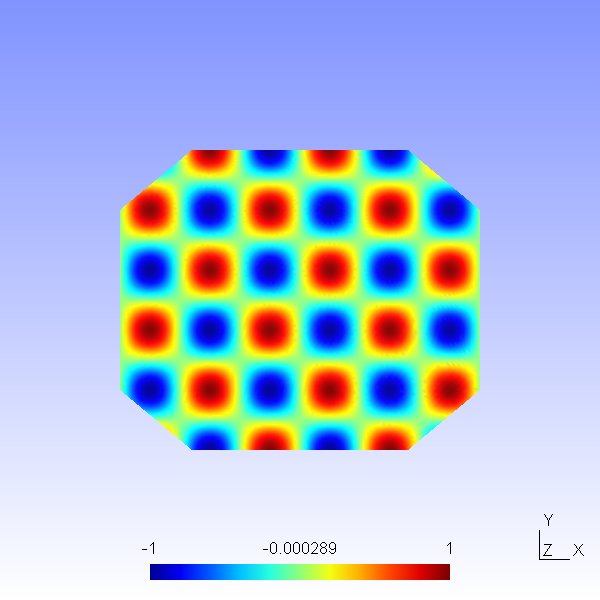
\includegraphics[width=6cm]{img/Helmholtz2D}
\caption{Solution of the 2D Helmholtz Problem.}
\label{f:adrsolver:helmholtz2D}
\end{center}
\end{figure}


\subsection{Advection dominated mass transport in a pipe}

The following example demonstrates the application of the ADRsolver for
modelling advection dominated mass transport in a straight pipe.
Such a transport regime is encountered frequently when modelling mass transport
in arteries. This is because the diffusion coefficient of small blood borne
molecules, for example oxygen or adenosine triphosphate, is very small
$O(10^{-10})$.

\subsubsection{Background}
The governing equation for modelling mass transport is the unsteady advection
diffusion equation:
\begin{align*}
\dfrac{\partial u}{\partial t}  + v\nabla u +  \epsilon \nabla^2 u = 0
\end{align*}

For small diffusion coefficient, $\epsilon$, the transport is dominated by
advection and this leads to a very fine boundary layer adjacent to the surface
which must be captured in order to get a realistic representation of the wall
mass transfer processes. This creates problems not only from a meshing
perspective, but also numerically where classical oscillations are observed in
the solution due to under-resolution of the boundary layer.

The Graetz-Nusselt solution is an analytical solution of a developing mass (or
heat) transfer boundary layer in a pipe. Previously this solution has been used
as a benchmark for the accuracy of numerical methods to capture the fine
boundary layer which develops for high Peclet number transport (the ratio of
advection to diffusion). The solution is derived based on the assumption that
the velocity field within the mass transfer boundary layer is linear i.e. the
Schmidt number (the relative thickness of the momentum to mass transfer boundary
layer) is sufficiently large. The analytical solution for the non-dimensional
mass transfer at the wall is given by:
\begin{align*}
S h(z) = \dfrac{2^{4/3}(Pe R/z)^{1/3}}{g^{1/3}\Gamma(4/3)} , 
\end{align*}
where $z$ is the streamwise coordinate, $R$ the pipe radius, $\Gamma(4/3)$ an incomplete 
Gamma function and $Pe$ the Peclet number given by:
\begin{align*}
Pe = \dfrac{2 U R}{\epsilon}
\end{align*}

In the following we will numerically solver mass transport in a pipe and compare
the calculated mass transfer at the wall with the Graetz-Nusselt solution. The
Peclet number of the transport regime under consideration is $750000$, which is
physiologically relevant.

\subsubsection{Input file}
The geometry under consideration is a pipe of radius, $R = 0.5$ and length $l =
0.5$

\begin{figure}[h!]
\begin{center}
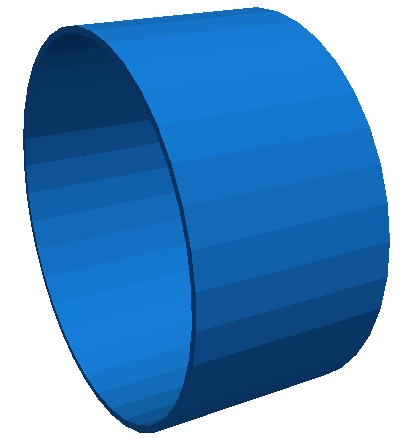
\includegraphics[width=6cm]{img/pipe}
\caption{Pipe.}
\end{center}
\end{figure}

Since the mass transport boundary layer will be confined to a very small layer
adjacent to the wall we do not need to mesh the interior region, hence the mesh
consists of a layer of ten prismatic elements over a thickness of 0.036R. The
elements progressively grow over the thickness of domain.

In this example we utilise heterogeneous polynomial order, in which the
polynomial order normal to the wall is higher so that we avoid unphysical
oscillations, and hence the incorrect solution, in the mass transport boundary
layer. To do this we specify explicitly the expansion type, points type and
distribution in each direction as follows:
\begin{lstlisting}[style=XMLStyle]
<EXPANSIONS>
  <E COMPOSITE="C[0]"
     NUMMODES="3,5,3"
     BASISTYPE="Modified_A,Modified_A,Modified_B"
     NUMPOINTS="4,6,3"
     POINTSTYPE="GaussLobattoLegendre,GaussLobattoLegendre,GaussRadauMAlpha1Beta0"
     FIELDS="u" />
</EXPANSIONS>
\end{lstlisting}

The above represents a quadratic polynomial order in the azimuthal and
streamwise direction and 4th order polynomial normal to the wall for a prismatic
element.

We choose to use a continuous projection and an first-order implicit-explicit
time-integration scheme. The \inltt{DiffusionAdvancement} and
\inltt{AdvectionAdvancement} parameters specify how these terms are treated.
\begin{lstlisting}[style=XMLStyle]
<I PROPERTY="EQTYPE"                VALUE="UnsteadyAdvectionDiffusion" />
<I PROPERTY="Projection"            VALUE="Continuous" />
<I PROPERTY="DiffusionAdvancement"  VALUE="Implicit" />
<I PROPERTY="AdvectionAdvancement"  VALUE="Explicit" />
<I PROPERTY="TimeIntegrationMethod" VALUE="IMEXOrder1" />
<I PROPERTY="GlobalSysSoln"         VALUE="IterativeStaticCond" />
\end{lstlisting}

We integrate for a total of $30$ time units with a time-step of $0.0005$,
necessary to keep the simulation numerically stable.
\begin{lstlisting}[style=XMLStyle]
<P> TimeStep = 0.0005              </P>
<P> FinalTime = 30                 </P>
<P> NumSteps = FinalTime/TimeStep  </P>
\end{lstlisting}

The value of the $\epsilon$ parameter is $\epsilon = 1/Pe$
\begin{lstlisting}[style=XMLStyle]
<P> epsilon = 1.33333e-6           </P>
\end{lstlisting}

The analytical solution represents a developing mass transfer boundary layer in
a pipe. In order to reproduce this numerically we assume that the inlet
concentration is a uniform value and the outer wall concentration is zero; this
will lead to the development of the mass transport boundary layer along the
length of the pipe. Since we do not model explicitly the mass transfer in the
interior region of the pipe we assume that the inner wall surface concentration
is the same as the inlet concentration; this assumption is valid based on the
large Peclet number meaning the concentration boundary layer is confined to the
region in the immediate vicinity of the wall. The boundary conditions are
specified as follows in the input file:
\begin{lstlisting}[style=XMLStyle]
<BOUNDARYREGIONS>
   <B ID="0"> C[3] </B>  <!-- inlet -->
   <B ID="1"> C[4] </B>  <!-- outlet -->
   <B ID="2"> C[2] </B>  <!-- outer surface -->
   <B ID="3"> C[5] </B>  <!-- inner surface -->
</BOUNDARYREGIONS>

<BOUNDARYCONDITIONS>
  <REGION REF="0">
    <D VAR="u" VALUE="1" />
  </REGION>
  <REGION REF="1">
    <N VAR="u" VALUE="0" />
  </REGION>
  <REGION REF="2">
    <D VAR="u" VALUE="0" />
  </REGION>
  <REGION REF="3">
    <D VAR="u" VALUE="1" />
  </REGION>
</BOUNDARYCONDITIONS>
\end{lstlisting}

The velocity field within the domain is fully devqeloped pipe flow (Poiseuille
flow), hence we can define this through an analytical function as follows:
\begin{lstlisting}[style=XMLStyle]
<FUNCTION NAME="AdvectionVelocity">
  <E VAR="Vx" VALUE="0" />
  <E VAR="Vy" VALUE="0" />
  <E VAR="Vz" VALUE="2.0*(1-(x*x+y*y)/0.25)" />
</FUNCTION>
\end{lstlisting}

We assume that the initial domain concentration is uniform everywhere and the
same as the inlet. This is defined by, 
\begin{lstlisting}[style=XMLStyle]
<FUNCTION NAME="InitialConditions">
  <E VAR="u" VALUE="1" />
</FUNCTION>
\end{lstlisting}

\subsubsection{Results}
To compare with the analytical expression we numerically calculate the
concentration gradient at the surface of the pipe. This is then plotted against
the analytical solution by extracting the solution along a line in the
streamwise direction, as shown in Fig.~\ref{f:adrsolver:masstransport}.

\begin{figure}[h!]
\begin{center}
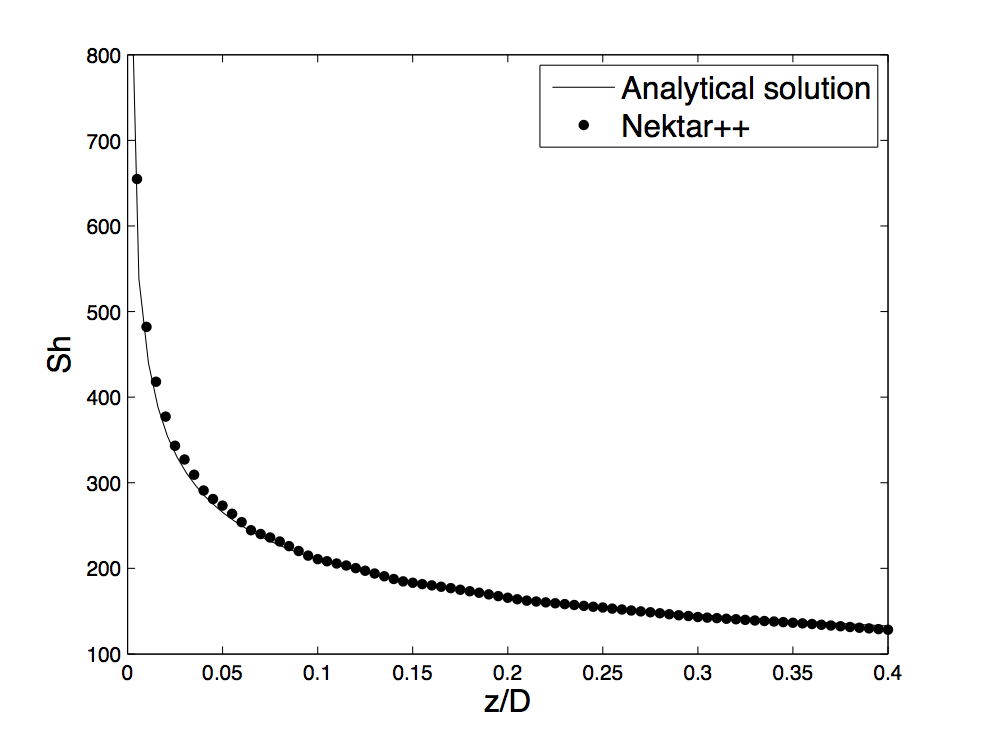
\includegraphics[width=7cm]{img/graetz-nusselt}
\caption{Concentration gradient at the surface of the pipe.}
\label{f:adrsolver:masstransport}
\end{center}
\end{figure}



